\chapter{实验研究示例章}
\label{chap:experiment}

本章展示实验研究部分的常见格式，包括实验设计、实验结果表格、实验数据图等。

\section{实验设计}
\subsection{实验目的}
本实验旨在验证相关理论分析的正确性，获取关键参数的实际数值。

\subsection{实验条件}
实验在标准实验室条件下进行，具体实验条件见表\ref{tab:experiment_conditions}。

\begin{table}[htbp]
    \caption{实验条件参数表}
    \label{tab:experiment_conditions}
    \centering
    \begin{tabular}{lll}
        \toprule
        参数类型 & 参数名称 & 参数值 \\
        \midrule
        环境参数 & 温度 & 25$\pm$2$^\circ$C \\
        环境参数 & 相对湿度 & 50$\pm$5\% \\
        设备参数 & 加载速率 & 1.0 mm/min \\
        设备参数 & 数据采集频率 & 100 Hz \\
        \bottomrule
    \end{tabular}
\end{table}

\subsection{试件信息}
本次实验共设计6个试件，试件基本信息见表\ref{tab:specimen_info}。

\begin{table}[htbp]
    \caption{试件基本信息表}
    \label{tab:specimen_info}
    \centering
    \begin{threeparttable}
    \begin{tabular}{C{2cm}C{3cm}C{3cm}C{3cm}}
        \toprule
        试件编号 & 尺寸参数(mm) & 材料类型 & 加载方式 \\
        \midrule
        Spec-1 & 200$\times$100$\times$10 & Type-A & 静态加载 \\
        Spec-2 & 200$\times$100$\times$10 & Type-A & 循环加载 \\
        Spec-3 & 300$\times$150$\times$15 & Type-B & 静态加载 \\
        Spec-4 & 300$\times$150$\times$15 & Type-B & 循环加载 \\
        Spec-5 & 400$\times$200$\times$20 & Type-C & 静态加载 \\
        Spec-6 & 400$\times$200$\times$20 & Type-C & 循环加载 \\
        \bottomrule
    \end{tabular}
    \begin{tablenotes}
        \footnotesize
        \item[*] 尺寸参数为试件的长度$\times$宽度$\times$厚度。
    \end{tablenotes}
    \end{threeparttable}
\end{table}

\section{实验结果}
\subsection{力学性能测试结果}
各试件的力学性能测试结果汇总于表\ref{tab:mechanical_results}。

\begin{table}[htbp]
    \caption{力学性能测试结果汇总表}
    \label{tab:mechanical_results}
    \centering
    \begin{tabular}{lcccc}
        \toprule
        试件编号 & 强度(MPa) & 延伸率(\%) & 弹性模量(GPa) & 破坏模式 \\
        \midrule
        Spec-1 & 350.5 & 12.3 & 210.0 & 拉断 \\
        Spec-2 & 340.2 & 15.1 & 205.5 & 疲劳 \\
        Spec-3 & 380.1 & 10.5 & 215.0 & 剪切 \\
        Spec-4 & 365.8 & 13.2 & 208.3 & 疲劳 \\
        Spec-5 & 420.3 & 8.5 & 220.0 & 弯曲 \\
        Spec-6 & 395.6 & 11.8 & 212.5 & 疲劳 \\
        \bottomrule
    \end{tabular}
\end{table}

\subsection{荷载-位移曲线}
荷载-位移曲线是实验结果的重要表现形式。
图\ref{fig:load_disp_curves}展示了荷载-位移曲线图的排版格式示例。
（注：此处使用神经网络图片作为格式占位示例，实际使用时请替换为真实的荷载-位移曲线图）

\begin{figure}[htbp]
    \centering
    \begin{subfigure}[b]{0.45\textwidth}
        \centering
        % 占位图片示例，请替换为实际的荷载-位移曲线图
        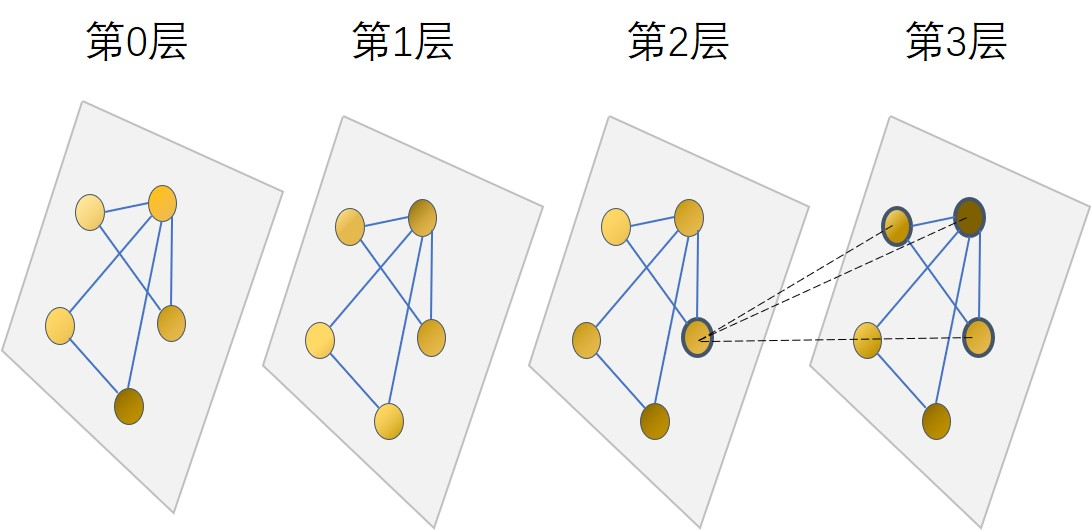
\includegraphics[width=\textwidth]{figures/GNN.jpg}
        \caption{静态加载试件（占位示例）}
    \end{subfigure}
    \hfill
    \begin{subfigure}[b]{0.45\textwidth}
        \centering
        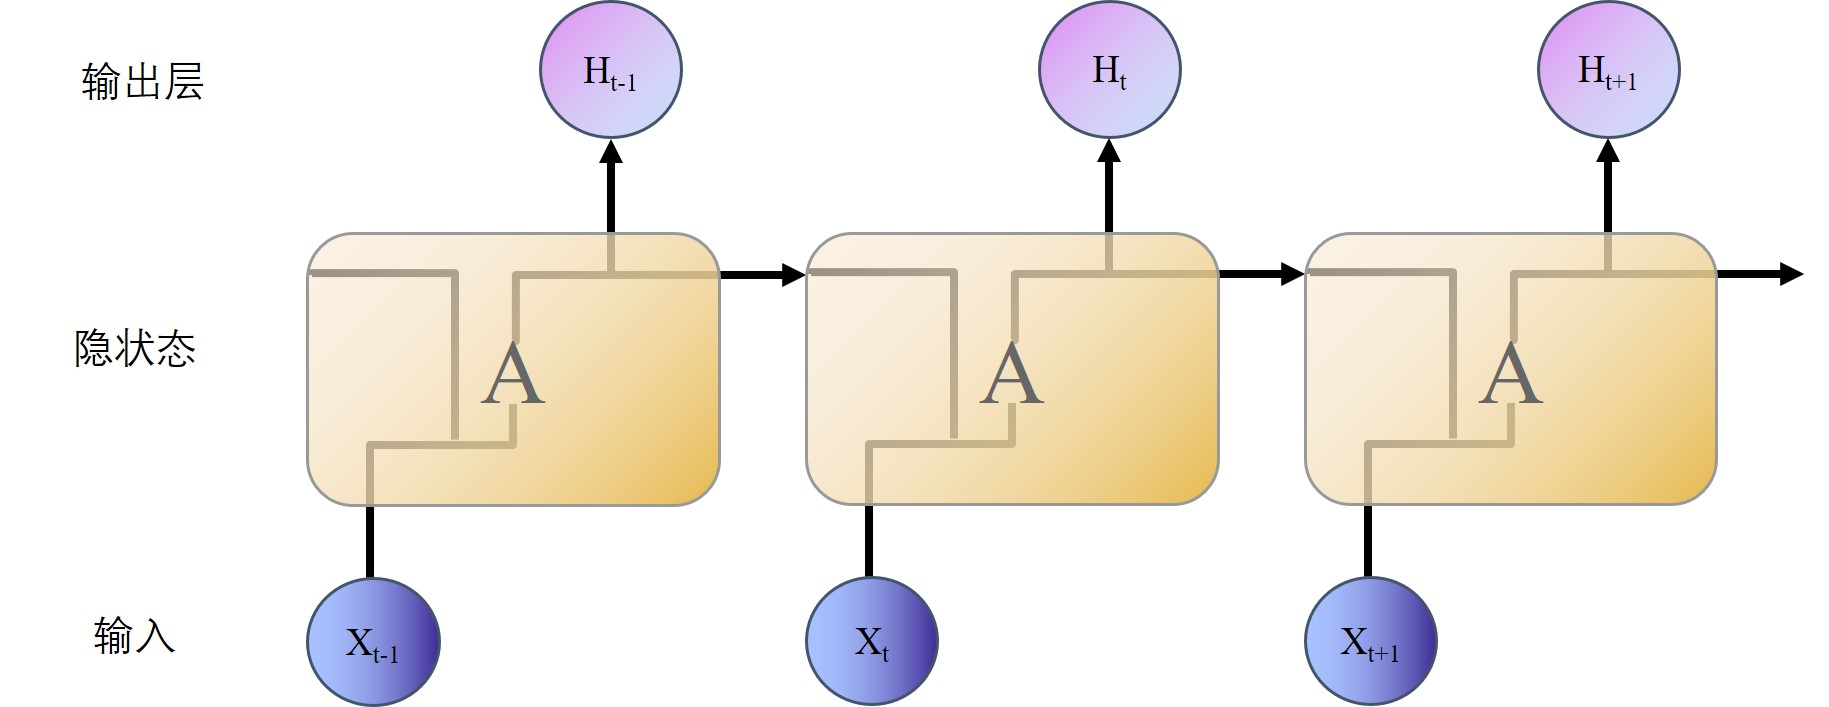
\includegraphics[width=\textwidth]{figures/RNN.jpg}
        \caption{循环加载试件（占位示例）}
    \end{subfigure}
    \caption{荷载-位移曲线排版格式示例（请替换为实际实验数据图）}
    \label{fig:load_disp_curves}
\end{figure}

\section{实验结果分析}
\subsection{强度分析}
从表\ref{tab:mechanical_results}可以看出，不同类型试件的强度存在明显差异。
Type-C试件强度最高，达到420.3 MPa，比Type-A试件高出约20\%。

\subsection{延伸率分析}
延伸率反映了材料的塑性变形能力。
循环加载试件的延伸率普遍高于静态加载试件。

\subsection{破坏模式分析}
不同加载方式下试件的破坏模式存在差异：
\begin{itemize}
    \item 静态加载试件主要表现为拉断、剪切或弯曲破坏；
    \item 循环加载试件主要表现为疲劳破坏。
\end{itemize}